\transitionFrame{Network Capacity \& Adversarial Robustness}

\begin{frame}
	\onslide<+->{Solving the following equation is not enough to guarantee the robustness and accuracy of the classifier.
		\begin{equation*}
		{\min_{\params} \rho(\params)}\text{, where } \rho(\params) = \mathbb{E}_{(\X,\y) \sim \distr} \sbrack{{ \max_{\delta \in \sPerturb} \loss (\X + \perturb, \y ; \params)}}
		\end{equation*}
	}

	\onslide<+->{The problem must have a small \colortext{green}{\textit{value}}, which means that the final loss achieved by the classifier against adversarial examples must be small.}
	
	\vspace{4pt}
	
	\onslide<+->{Therefore, a very small \colortext{blue}{$\rho(\params)$} corresponds to a perfect classifier that is robust to adversarial inputs.}
	
	\vspace{4pt}
	
	\onslide<+->{For a fixed set $\perturb$, the value of the problem is entirely dependent on the
		architecture of the classifier.}
	
	\vspace{4pt}
	
	\onslide<+->{Therefore, the architectural capacity of the model is very important for its over performance.}
\end{frame}

\begin{frame}{Visualizing the Effect of Capacity}
	\begin{columns}
		\begin{column}{0.32\textwidth}
			\onslide<+->{
				\begin{center}
					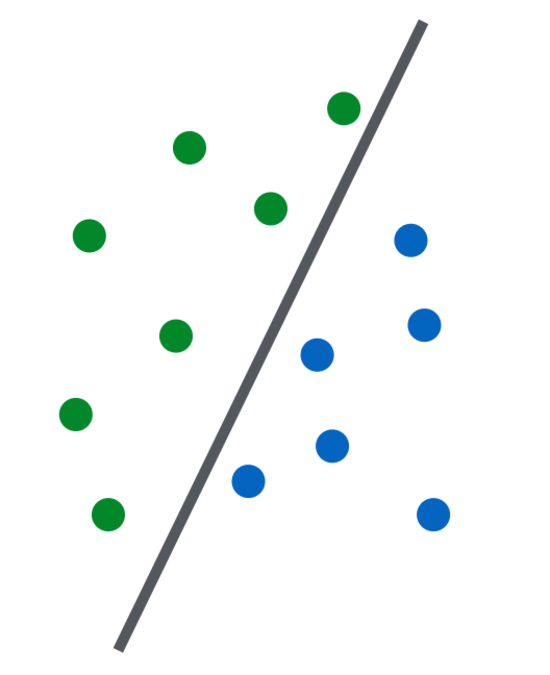
\includegraphics[scale=0.3]{capacity/benign_only.pdf}
					
					(Benign) binary classification using a \\\blue{linear decision boundary}
				\end{center}
			}
		\end{column}
		\begin{column}{0.32\textwidth}
			\onslide<+->{
				\begin{center}
					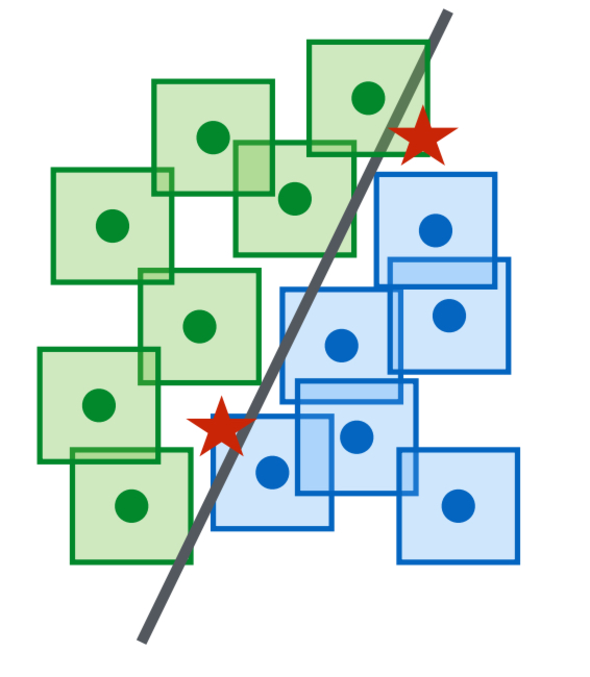
\includegraphics[scale=0.3]{capacity/misclassified_adv.pdf}
					
					Adversarial $\ell_{\infty}$ balls
					\\
					\red{$\star$} misclassified \\ adversarial examples
				\end{center}
			}
		\end{column}
		\begin{column}{0.32\textwidth}
			\onslide<+->{
				\begin{center}
					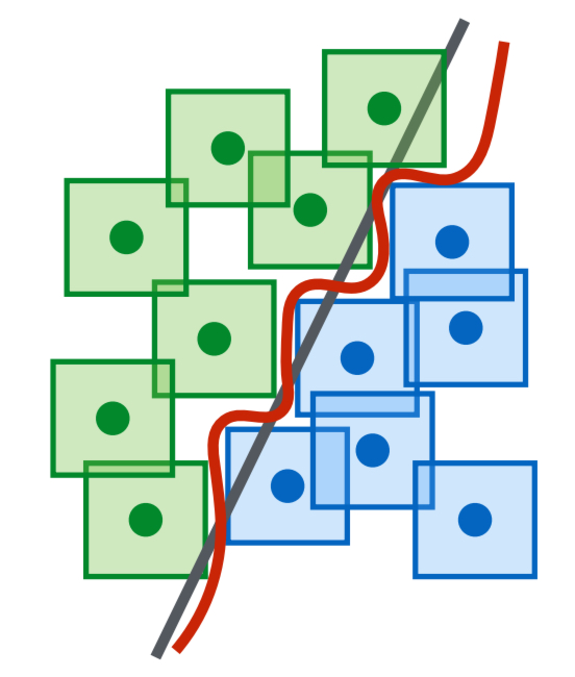
\includegraphics[scale=0.3]{capacity/complicated_decision.pdf}
					
					``Complicated'' decision boundary required
				\end{center}
			}
		\end{column}
	\end{columns}
\end{frame}

\begin{frame}{}
	\begin{columns}
		\begin{column}{0.48\textwidth}
			\onslide<+->{
				\begin{center}
					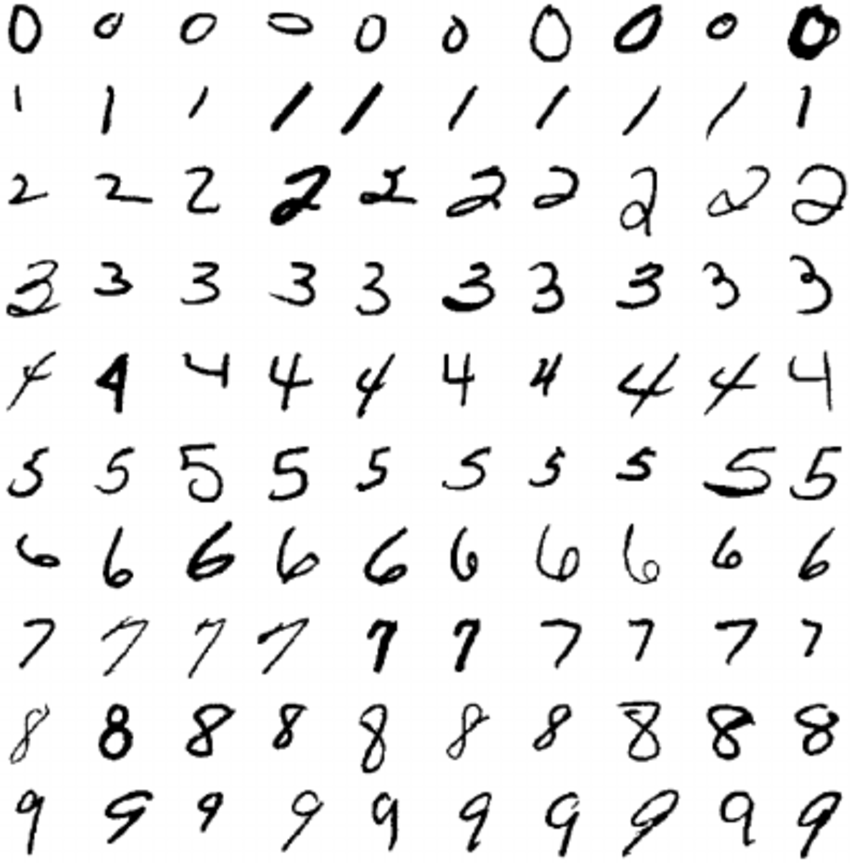
\includegraphics[scale=0.18]{nc_ar/mnist.png}
					
					MNIST
				\end{center}
			}
		\end{column}
		\begin{column}{0.48\textwidth}
			\onslide<+->{
				\begin{center}
					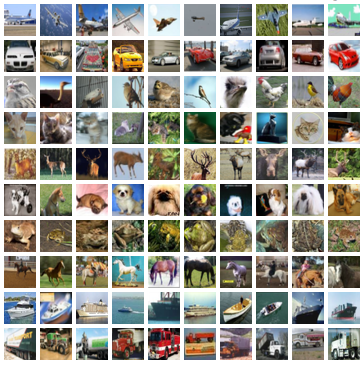
\includegraphics[scale=0.44]{nc_ar/cifar10.png}
					
					CIFAR10
				\end{center}
			}
		\end{column}
	\end{columns}
\end{frame}

\begin{frame}
	\onslide<+->{Verified by their experiments, capacity is crucial for:
		\begin{itemize}[<+->]
			\setlength\itemsep{8pt}
			\item Robustness
			\item The ability to successfully train a classifier against strong adversaries. 
		\end{itemize}
	}
	\begin{columns}
		\begin{column}{0.99\textwidth}
			\onslide<+->{
				\begin{center}
					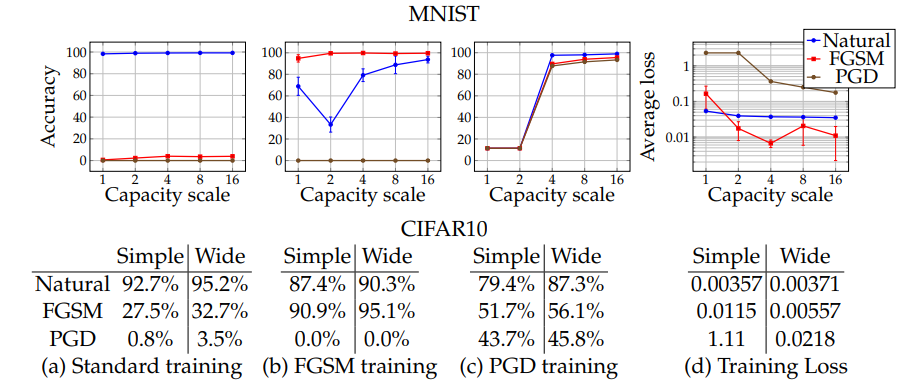
\includegraphics[scale=0.38]{nc_ar/fig4.png}
				\end{center}
			}
		\end{column}
	\end{columns}
\end{frame}

\begin{frame}
	\onslide<+->{What they found:
		\begin{itemize}[<+->]
			\setlength\itemsep{8pt}
			\item Capacity alone helps
			\item FGSM adversaries don’t increase robustness (for large  $\varepsilon$)
			\item Weak models may fail to learn non-trivial classifiers
			\item The value of the saddle point problem decreases as we increase the capacity
			\item More capacity and stronger adversaries decrease transferability
		\end{itemize}
	}
\end{frame}

\subsection{Experiments}
\begin{frame}
	\onslide<+->{Two key elements in training their robust classifiers
		\begin{itemize}[<+->]
			\setlength\itemsep{8pt}
			\item A sufficiently high capacity network
			\item The strongest possible adversary
		\end{itemize}
	}
	\vspace{15pt}
	\onslide<+->{Using a "complete" first-order adversary by PGD for both MNIST and CIFAR10:
		\begin{itemize}[<+->]
			\setlength\itemsep{8pt}
			\item Multiple epochs for training the model. Therefore, no benefit from restarting PGD multiple times per batch
		\end{itemize}
	}
\end{frame}


\begin{frame}
	The steady decrease in the training loss of adversarial examples indicates successfully solution for the original optimization problem during training.

	\begin{columns}
		\begin{column}{0.99\textwidth}
			\onslide<+->{
				\begin{center}
					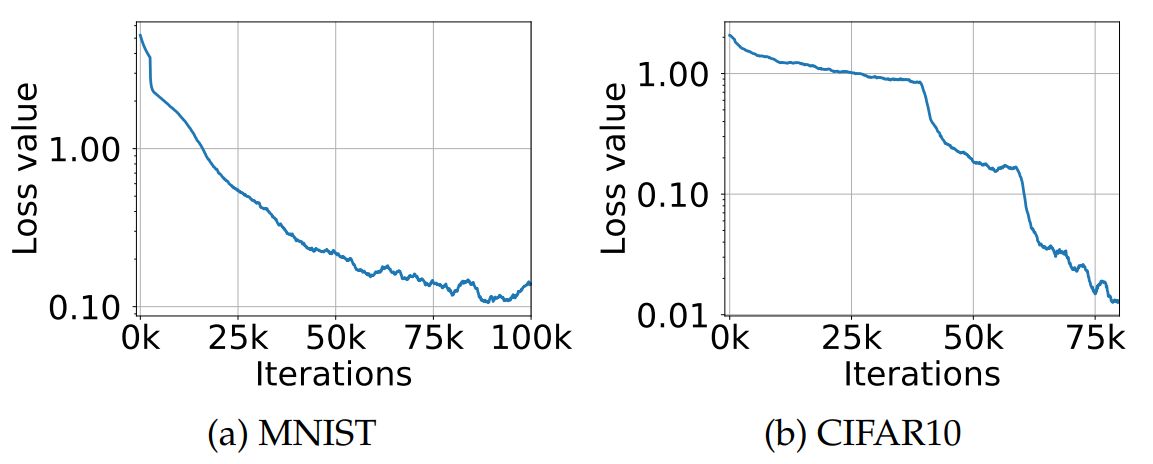
\includegraphics[scale=0.3]{nc_ar/fig5.png}
				\end{center}
			}
		\end{column}
	\end{columns}
\end{frame}

\begin{frame}
	\onslide<+->{Models are trained against a range of adversaries:
		\begin{itemize}[<+->]
			\setlength\itemsep{8pt}
			\item White-box attacks with PGD for a different number of iterations and restarts (A)
			\item White-box attacks with PGD using the Carlini-Wagner (CW), and CW+ when ${\kappa = 50}$
			\item Black-box attacks from an independently trained copy of the network (A$^{'}$).
			\item Black-box attacks from a version of the same network trained only on natural examples (A$_{nat}$)
			\item Black-box attacks from a different convolution architecture (B)
		\end{itemize}
	}
\end{frame}

\begin{frame}
	\begin{columns}
		\begin{column}{0.99\textwidth}
			\onslide<+->{
				\begin{center}
					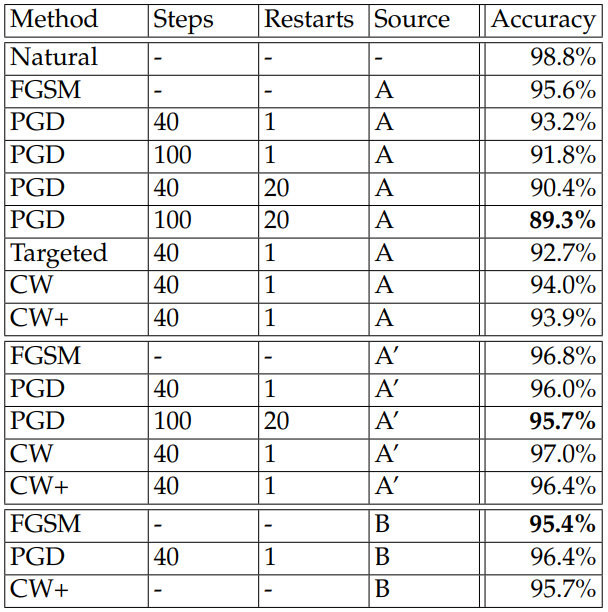
\includegraphics[scale=0.3]{nc_ar/table1.png}
				\end{center}
			}
		\end{column}
	\end{columns}
\end{frame}

\begin{frame}
	\begin{columns}
		\begin{column}{0.99\textwidth}
			\onslide<+->{
				\begin{center}
					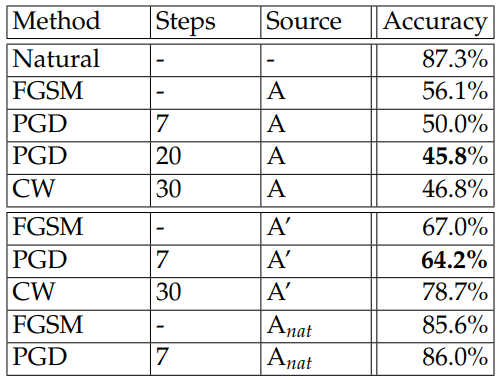
\includegraphics[scale=0.3]{nc_ar/table2.png}
				\end{center}
			}
		\end{column}
	\end{columns}
\end{frame}

\begin{frame}
	\begin{columns}
		\begin{column}{0.99\textwidth}
			\onslide<+->{
				\begin{center}
					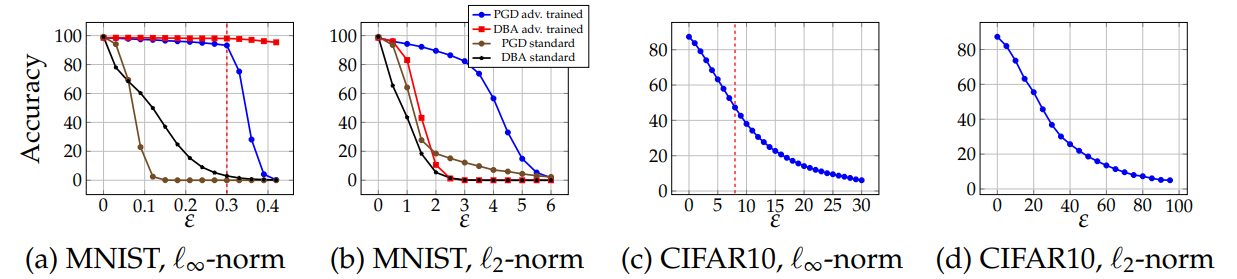
\includegraphics[scale=0.3]{nc_ar/fig6.png}
				\end{center}
			}
		\end{column}
	\end{columns}
\end{frame}

\begin{frame}
	\onslide<+->{Conclusion:
		\begin{itemize}[<+->]
			\setlength\itemsep{15pt}
			\item Although deep neural networks very vulnerable to adversarial attacks, they can be made resistant to adversarial attacks
			\item Based on the theory and experiments, reliable adversarial training methods can be designed because of the unexpectedly regular structure of the underlying optimization task:
			\begin{itemize}[<+->]
				\setlength\itemsep{15pt}
				\item Even though the relevant problem corresponds to the maximization of a highly
				non-concave function with many distinct local maxima, their values are highly concentrated.
			\end{itemize}
		\end{itemize}
	}
\end{frame}

\section{Related Works}
\begin{frame}
	\begin{itemize}[<+->]
		\setlength\itemsep{15pt}
		\item Robust optimization, not a new topic
		\item Adversarial ML, not a new topic
		\item Having the above in the context of DNN is their contribution
	\end{itemize}

	\onslide<+->{
		Recent work on adversarial training on ImageNet also observed that the model capacity is important for adversarial training. Their contribution
		\begin{itemize}[<+->]
			\setlength\itemsep{15pt}
			\item Training against multi-step methods (PGD) does lead to resistance against adversaries
		\end{itemize}
	}
\end{frame}

\begin{frame}
	\onslide<+->{
		There are previous works on the min-max optimization problem. But, there are three differences:
		\begin{itemize}[<+->]
			\setlength\itemsep{15pt}
			\item (Previous works) the inner maximization problem can be difficult to solve, (they) it
			is possible to obtain sufficiently good solutions using randomly re-started projected gradient descent 
			\item (Previous works) one-step adversaries, (they) multi-step methods
			\item (Previous works)  FGSM --FGSM-only evaluations are not fully reliable, (they) PGD
		\end{itemize}
	}
\end{frame}